\chapter{Quantum walks}

In classical random walks, the walker moves from the current vertex via one of its outgoing edges, chosen randomly, weighted by the edge weights. This random choice can be interpreted as a (generalized) coin toss.

To formulate a quantum version of graph walking, we define the quantum coin, which will replace the classical concept of randomness with quantum superposition.

\section{Formulating the Quantum coin}

I used Renato Portugal's Quantum Walks and Search Algorithms~\cite{Portugal} book as a reference for the different types of coins I present in this section.

A \textit{quantum coin} is a quantum system, which behaves according to the postulates of quantum mechanics. It has a current state, represented by a state vector in a Hilbert space and a unitary time evolution operator, describing a coin toss.

After tossing the coin, the resulting coin state chooses the next step of the quantum walker. If there are $d$ outgoing edges to choose from, then the coin's state space must have $d$ orthonormal basis states, each corresponding to one of the possible edges. If the current state is one of the basis states, then the walker moves in that direction. However, in the quantum world, the coin can also be in a superposition, consisting of multiple basis states. This means that the walker will simultaneously move in all corresponding directions and occupy more than one vertex at the same time, resulting in the walker spreading over the graph in a superposition.

For the $d$ dimensional coin state, the corresponding coin flip operator is a $(d\times{}d)$ dimensional unitary matrix. Based on what the transition operator is, multiple types of coins can be defined. The following ones are typically used in quantum walks.

\subsection{Hadamard coin}

The Hadamard coin is the most commonly used quantum coin. It is defined by the Hadamard-matrix as a transition operator:

\begin{align*}
  \mathbf{H} = \frac{1}{\sqrt{2}}\begin{pmatrix}
      1 & 1  \\
      1 & -1
    \end{pmatrix}.
\end{align*}

If the starting coin state is $\ket{0}$, then flipping the coin once results in the following state:

\begin{align*}
 \mathbf{H}\ket{0} = \frac{1}{\sqrt{2}}\begin{pmatrix}
      1 & 1  \\
      1 & -1
    \end{pmatrix} \begin{pmatrix} 1 \\ 0 \end{pmatrix}
    = \frac{1}{\sqrt{2}} \begin{pmatrix} 1 \\ 1 \end{pmatrix} = \frac{1}{\sqrt{2}} \ket{0} + \frac{1}{\sqrt{2}} \ket{1}.
\end{align*}

If we measured the above coin, the probability of measuring $0$ is

\begin{align*}
P(0 \mid \frac{1}{\sqrt{2}} (\ket{0} + \ket{1})) =
\left\lvert\frac{1}{\sqrt{2}}\right\rvert^2 =
\frac{1}{2}.
\end{align*}

Similarly, if the starting coin state is $\ket{1}$, then flipping the coin once results in the following state:

\begin{align*}
   \mathbf{H}\ket{1} = \frac{1}{\sqrt{2}}\begin{pmatrix}
      1 & 1  \\
      1 & -1
    \end{pmatrix} \begin{pmatrix} 0 \\ 1 \end{pmatrix}
    = \frac{1}{\sqrt{2}} \begin{pmatrix} 1 \\ -1 \end{pmatrix} = \frac{1}{\sqrt{2}} \ket{0} - \frac{1}{\sqrt{2}} \ket{1}.
\end{align*}

The probability of measuring $1$ here is similarly

\begin{align*}
P(1 \mid \frac{1}{\sqrt{2}} (\ket{0} - \ket{1})) =
\left\lvert-\frac{1}{\sqrt{2}}\right\rvert^2 =
\frac{1}{2}.
\end{align*}

An unexpected feature of this coin comes from the fact, that the Hadamard-matrix is Hermitian (self-adjoint), i.e. $\mathbf{H}^{\dagger} = \mathbf{H}$, while also unitary, i.e. $\mathbf{H}^{\dagger} = \mathbf{H}^{-1}$, which results in $\mathbf{H}^{-1} = \mathbf{H}$, thus $\mathbf{H}\mathbf{H} = \mathbf{I}$. This means, that after flipping the coin twice without measuring it, it will return the coin state to its origin. For example, starting from $\ket{0}$:

\begin{align*}
 \mathbf{H}^2 \ket{0} = \mathbf{H}\frac{1}{\sqrt{2}}(\ket{0} + \ket{1}) = \frac{1}{2}(\ket{0} + \ket{1} + \ket{0} - \ket{1}) = \ket{0}.
\end{align*}

After the second flip, the probability of measuring $\ket{0}$ is $1$, due to the destructive interference between the two $\ket{1}$ probability amplitudes, demonstrating a significant contrast between classical and quantum walks.

\begin{definition}[$2^n$ dimensional Hadamard-coin]

A $2^n$ dimensional Hadamard-coin operator can be created by taking the tensor product of the $2$ dimensional Hadamard-coin $n$ times: $\mathbf{H}^{\otimes{}n}$.

\end{definition}

\subsection{Grover coin}

The Grover coin originates from Grover's search algorithm, where it is applied as the diffusion operator.

Let $\ket{D}$ be the following state:

\begin{align*}
\ket{D} = \mathbf{H}^{\otimes{}n}\ket{0} =
\frac{1}{\sqrt{2^n}} \sum\limits_{i=0}^{2^n-1} \ket{i}.
\end{align*}

Using $\ket{D}$, the Grover coin is the following unitary matrix:

\begin{align*}
    \mathbf{G} = 2\ket{D}\bra{D} - \mathbf{I}.
\end{align*}

If $N = 2^n$, then $\mathbf{G}$ unrolls to the following representation:

\begin{align*}
  \mathbf{G} = \begin{pmatrix}
      \frac{2}{N} - 1 & \frac{2}{N} & \dots  & \frac{2}{N} \\
      \frac{2}{N} & \frac{2}{N} - 1 & \dots  & \frac{2}{N} \\
      \vdots & \vdots & \ddots & \vdots \\
      \frac{2}{N} & \frac{2}{N} & \ddots & \frac{2}{N} - 1
    \end{pmatrix}.
\end{align*}

\subsection{Fourier coin}

In contrast to the Hadamard and Grover coins, the Fourier coin can be of any size, not just a power of 2. A size $N$ Fourier-coin, $F_N$ is defined by the matrix of the Quantum Fourier Transform:

\begin{align*}
\mathbf{F}[k,l] = \frac{1}{\sqrt{N}} \omega^{kl}
\end{align*}

where $\omega$ is the $N$-th root of unity,

\begin{align*}
\omega = e^{\frac{2\pi{}i}{N}}.
\end{align*}

$\mathbf{F}$ unrolls to the following representation:

\begin{align*}
\mathbf{F} = \frac{1}{\sqrt{N}}
\begin{pmatrix}
  1 & 1 & 1 & \dots & 1 \\
  1 & \omega & \omega^2 & \dots & \omega^{N-1} \\
  1 & \omega^2 & \omega^4 & \dots & \omega^{2(N-1)} \\
  \vdots & \vdots & \vdots & \ddots & \vdots \\
  1 & \omega^{N-1} & \omega^{2(N-1)} & \dots & \omega^{(N-1)(N-1)}
\end{pmatrix}
\end{align*}

\section{Quantum walks on the line}

Kempe introduces quantum walks from a physicist's perspective in~\cite{KempeIntroduction} using a particle characterised by its position on the line $\ket{x}$ and its spin state $\ket{s}$.

\subsection{State space}

\lineparagraph{Spin state}

The spin state is in $H_2$ with the basis states spin up and down:

\begin{align*}
\ket{\uparrow} = \ket{0}, \\
\ket{\downarrow} = \ket{1}.
\end{align*}

The spin state vector is then given by:

\begin{align*}
\ket{s} = s_0 \ket{\uparrow} + s_1 \ket{\downarrow}.
\end{align*}

\lineparagraph{Position state}

At the start of the walk the particle is at the origin $\ket{0}$ and the walking lasts for $N$ steps. The position state is in $H_{(2N+1)}$ with the following basis vectors corresponding to the possible positions on the line.

\begin{align*}
\{
\ket{-N},\ket{-(N-1)},\dots,
\ket{-1},\ket{0},\ket{1},\dots,
\ket{N-1},\ket{N}
\}
\end{align*}

I index the basis states using negative numbers to match the labels on the axis.

The position state vector is then given by:

\begin{align*}
    \ket{x} = \sum\limits_{i=-N}^{N}x_i\ket{i}.
\end{align*}

\lineparagraph{Composite state}

The composite state of the system, according to \hyperref[PostulateIV]{[PostulateIV]} is then

\begin{align*}
    \ket{x}\otimes{}\ket{s}.
\end{align*}

\subsection{Evolution}

The particle travels on the line based on its current spin state:
\begin{itemize}
\item If the current spin state is $\ket{0}$, the particle moves to the left, i.e. from position $\ket{i}$ the particle travels to position $\ket{i-1}$.
\item If the current spin state is $\ket{1}$, the particle moves to the right, i.e. from position $\ket{i}$ the particle travels to position $\ket{i+1}$.
\end{itemize}

This step is realised with the unitary matrix $\mathbf{S}$ which operates on the complete state of the system, $\ket{x}\otimes{}\ket{s}$ and is assembled from a left and a right shift operator acting on $\ket{x}$ and another operator for checking $\ket{s}$ compiled using tensor product.

\begin{definition}[Left shift operator]

To move from position $\ket{i}$ to the left ($\ket{i-1}$) the position vector is multiplied with the following $\mathbf{L}$ matrix, containing $1$'s above the diagonal. To keep $\mathbf{S}$ unitary, an unused transition must be added in the lower left corner.

\change{Előrehivatkozni a permutációmátrixos tételre.}

\begin{align*}
\mathbf{L} = \ket{N}\bra{-N} + \sum\limits_{i=-(N-1)}^{N} \ket{i-1}\bra{i} =
\left(
    \begin{array}{ccccc}
        0      & 1      & 0      & \cdots & 0      \\
               & \ddots & \ddots & \ddots & \vdots \\
        \vdots &        & \ddots & \ddots & 0      \\
        0      &        &        & \ddots & 1      \\
        1      & 0      & \cdots &        & 0
      \end{array}
\right)
\end{align*}

For a given basis vector $\ket{j}$ only one of the summands in $\mathbf{L}$ is non-zero, where $i=j$, resulting in the required shift being performed.

\begin{align*}
\mathbf{L}\ket{j} = \ket{j-1}\bra{j}\ket{j} = \ket{j-1}
\end{align*}

\end{definition}

\begin{definition}[Right shift operator]

To move from position $\ket{i}$ to the right ($\ket{i+1}$) the position vector is multiplied with the following $\mathbf{R}$ matrix, containing $1$'s under the diagonal. To keep $\mathbf{S}$ unitary, an unused transition must be added in the top right corner.

\change{Előrehivatkozni a permutációmátrixos tételre.}

\begin{align*}
\mathbf{R} = \ket{-N}\bra{N} + \sum\limits_{i=-N}^{N-1} \ket{i+1}\bra{i} =
\left(
    \begin{array}{ccccc}
        0      &        & \cdots & 0      & 1      \\
        1      & \ddots &        &        & 0      \\
        0      & \ddots & \ddots &        & \vdots \\
        \vdots & \ddots & \ddots & \ddots &        \\
        0      & \cdots & 0      & 1      & 0
      \end{array}
\right)
\end{align*}

For a given basis vector $\ket{j}$ only one of the summands in $\mathbf{R}$ is non-zero, where $i=j$, resulting in the required shift being performed.

\begin{align*}
\mathbf{R}\ket{j} = \ket{j+1}\bra{j}\ket{j} = \ket{j+1}
\end{align*}

\end{definition}

\lineparagraph{Shift operator}

Using matrixes $L$ and $R$ operating on the position register $\ket{x}$ only, we construct a unitary operator $S$, which operates on the composite state of the system, $\ket{x} \otimes \ket{s}$, executing matrix $\mathbf{L}$ on $\ket{x}$ only when $\ket{s} = \ket{0}$ and matrix $\mathbf{R}$ only when $\ket{s}=\ket{1}$.

\begin{align*}
  \mathbf{S} = \mathbf{L}\otimes\ket{0}\bra{0} + \mathbf{R}\otimes\ket{1}\bra{1}
\end{align*}

The execution logic is as follows:

\begin{gather*}
    \mathbf{S}(\ket{x}\otimes{}\ket{s}) = \\
    (\mathbf{L}\otimes\ket{0}\bra{0} + \mathbf{R}\otimes\ket{1}\bra{1})(\ket{x}\otimes{}\ket{s}) = \\ (\mathbf{L}\otimes\ket{0}\bra{0})(\ket{x}\otimes{}\ket{s}) + (\mathbf{R}\otimes\ket{1}\bra{1})(\ket{x}\otimes{}\ket{s}) = \dots
\end{gather*}

using \hyperref[TensorDistributivity]{[TensorDistributivity]}:

\begin{gather*}
    \dots = \mathbf{L}\ket{x}\otimes(\ket{0}\bra{0}\ket{s}) + \mathbf{R}\ket{x}\otimes(\ket{1}\bra{1}\ket{s}) = \\
    \ket{x-1}\otimes{}s_0\ket{0} + \ket{x+1}\otimes{}s_1\ket{1} = \\
    s_0\ket{x-1, 0} + s_1\ket{x+1,1}.
\end{gather*}

\begin{itemize}
\item If the spin state was $\ket{s} = \ket{0}$ at the beginning, then $s_0=1$ and $s_1=0$, which means that the resulting system state is $\ket{x-1,0}$, which means that the particle shifted to the left, as designed.
\item If the spin state was $\ket{s} = \ket{1}$ at the beginning, then $s_0=0$ and $s_1=1$, which means that the resulting system state is $\ket{x+1,1}$, which means that the particle shifted to the right, also as intended.
\end{itemize}

Furthermore, the spin state can be any mixed state $s_0\ket{0} + s_1\ket{1}$ as well. In this case the particle will shift \textit{both} to the left and to the right, at the same time. When measured, the particle can be found in position $\ket{x-1}$ with probability $|s_0|^2$ and in position $\ket{x+1}$ with probability $|s_1|^2$.

In quantum graph walks, the walker can simultaneously explore multiple parallel paths in the graph, at the same time. With good design, this behaviour can be used to search the graph faster than in classical random graph walks.

\lineparagraph{Coin operator}

To inject the quantum superposition into the walk, the particle's spin state is transformed using any $2$ dimensional unitary matrix between shift operations. The Hadamard, Grover and Fourier coins mentioned earlier are commonly used as coin operators.

For any $C$ operator on the coin register, the unitary transform for the composite system is defined as follows:

\begin{align*}
    \hat{C} = I \otimes C
\end{align*}

since the coin operator does not modify the position register.

\lineparagraph{Complete step operator}

One step of the quantum walk on the line consists of flipping the coin once, then applying the shift operator, as follows:

\begin{align*}
    U = S\hat{C} = S(I\otimes{}C)
\end{align*}

\subsection{Measurement}

To measure the probability of the particle being at position $\ket{i}$, the projective measurement operator acting on $\ket{x}$ is defined as $P_i = \ket{i}\bra{i}$, in accordance with \hyperref[PostulateIIIProjective]{[PostulateIIIProjective]}.

Since the coin register need not be measured, we apply the identity operator on it, using $P_i \otimes I$ on the complete system to measure the particle's current position.

The probability of finding the particle in position $i$ is:

\begin{gather*}
    P(i | \ket{x}) = \bra{x,s}P_i\otimes{}I\ket{x,s} = \dots
\end{gather*}

using \hyperref[TensorDistributivity]{[TensorDistributivity]}:

\begin{gather*}
    \dots = \bra{x}P_i\ket{x}\bra{s}I\ket{s} =
    \bra{x}P_i\ket{x}1 =
    \bra{x}P_i\ket{x} =
    \bra{x}\ket{i}\bra{i}\ket{x} =
    |\bra{i}\ket{x}|^2 =
    |x_i|^2
\end{gather*}


\section{Generalization of Quantum Walks}

There are two ways to generalize quantum walking on the line to higher dimensional grids.

\begin{enumerate}
    \item \textbf{Use multiple independent 2 dimensional coins}: In~\cite{Portugal}, Renato Portugal describes the generalization of a quantum walk on a line to a 2 dimensional grid, using this technique with two independent walks on the $x$ and $y$ axes. In this work I will show the generalization technique for arbitrarily large dimensional grids.
    \item \textbf{Use a single higher dimensional coin}: In~\cite{Portugal}, Renato Portugal describes the generalization of a quantum walk on a line to an arbitrary undirected graph and gives the necessary condition for the creation of the unitary transition matrix, without proof. In this work I generalize to directed graphs and give proof of the generalization of the condition using directed graphs.
\end{enumerate}

\subsection{Generalization using multiple independent 2 dimensional coins}

\subsubsection{Quantum Walk on a 2D grid}

Legyen a rács $N = n \times n$ -es.

Pozíció vektor: $\ket{P} =  (p_{0}, \dots, p_{N})$, ahol
$p_{i}\in\mathds{C}$ ahol $0 \leq{} i < N$, $\forall{}i$-re és $\sum\limits_{i=0}^{N} |p_i|^2 = 1$.

\begin{align}
  \ket{P_{0}} =  (0, \dots, 0, 1, 0, \dots, 0)
\end{align}

\begin{align}
  C = (\frac{1}{\sqrt{2}}, \frac{i}{\sqrt{2}}) \otimes (\frac{1}{\sqrt{2}}, \frac{i}{\sqrt{2}})
\end{align}

\begin{align}
  S_{\text{left}} =
  \begin{pmatrix}
    0      & 0      & 0      & \dots  & 0 \\
    1      & 0      & 0      & \dots  & 0 \\
    0      & 1      & 0      & \ddots & 0 \\
    \vdots & \ddots & \ddots & 0
  \end{pmatrix}
\end{align}


\begin{align}
  L = U^{T}
\end{align}


\begin{itemize}
  \item Rács = két körnek a tenzorszorzata.
  \item Fel/le = mindig 1 sorral felette/alatta lévő (modulóval) van összekötve = n-el van elcsúsztatva.
  \item Függőlegesen számozva ugyanígy csak fordított elnevezések.
  \item Jobbra-balra = 1 távolság, kivéve sor végén, ahol a sor elejére ugrik = kis körök.
  \item Tenzorszorzás tulajdonságait előre kiszedni, műveletek, használatkor hivatkozni.
  \item Többsoros képleteknek csak 1 száma legyen.
\end{itemize}

\section{Példa}

\begin{align}
  n = 3
\end{align}

\begin{figure}[!ht]
  \begin{center}
    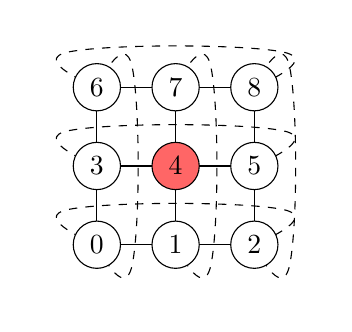
\begin{tikzpicture}

      \draw(0,0) -- (0,2);
      \draw(1,0) -- (1,2);
      \draw(2,0) -- (2,2);

      \draw [black, dashed] plot [smooth, tension=0.8] coordinates { (0,0) (0.45,-0.25) (0.45,2.25) (0,2)};
      \draw [black, dashed] plot [smooth, tension=0.8] coordinates { (1,0) (1.45,-0.25) (1.45,2.25) (1,2)};
      \draw [black, dashed] plot [smooth, tension=0.8] coordinates { (2,0) (2.45,-0.25) (2.45,2.25) (2,2)};


      \draw(0,0) -- (2,0);
      \draw(0,1) -- (2,1);
      \draw(0,2) -- (2,2);

      \draw [black, dashed] plot [smooth, tension=0.8] coordinates { (0,0) (-0.35,0.45) (2.35,0.45) (2,0)};
      \draw [black, dashed] plot [smooth, tension=0.8] coordinates { (0,1) (-0.35,1.45) (2.35,1.45) (2,1)};
      \draw [black, dashed] plot [smooth, tension=0.8] coordinates { (0,2) (-0.35,2.45) (2.35,2.45) (2,2)};

      \draw[black,fill=white](0,0) circle (0.3) node {0};
      \draw[black,fill=white](1,0) circle (0.3) node {1};
      \draw[black,fill=white](2,0) circle (0.3) node {2};

      \draw[black,fill=white](0,1) circle (0.3) node {3};
      \draw[black,fill=red!60](1,1) circle (0.3) node {4};
      \draw[black,fill=white](2,1) circle (0.3) node {5};

      \draw[black,fill=white](0,2) circle (0.3) node {6};
      \draw[black,fill=white](1,2) circle (0.3) node {7};
      \draw[black,fill=white](2,2) circle (0.3) node {8};

    \end{tikzpicture}
  \end{center}
  \caption{n=3-ös rács}
  \label{fig:3Racs}
\end{figure}

\begin{align}
  N = n^2 = 9
\end{align}

\begin{align}
  S_{\text{left}} = I_3 \otimes U_3 =
  \begin{pmatrix}
    0                  & \textcolor{red}{1} & 0                  & 0                  & 0                  & 0                  & 0                  & 0                  & 0                  \\
    0                  & 0                  & \textcolor{red}{1} & 0                  & 0                  & 0                  & 0                  & 0                  & 0                  \\
    \textcolor{red}{1} & 0                  & 0                  & 0                  & 0                  & 0                  & 0                  & 0                  & 0                  \\
    0                  & 0                  & 0                  & 0                  & \textcolor{red}{1} & 0                  & 0                  & 0                  & 0                  \\
    0                  & 0                  & 0                  & 0                  & 0                  & \textcolor{red}{1} & 0                  & 0                  & 0                  \\
    0                  & 0                  & 0                  & \textcolor{red}{1} & 0                  & 0                  & 0                  & 0                  & 0                  \\
    0                  & 0                  & 0                  & 0                  & 0                  & 0                  & 0                  & \textcolor{red}{1} & 0                  \\
    0                  & 0                  & 0                  & 0                  & 0                  & 0                  & 0                  & 0                  & \textcolor{red}{1} \\
    0                  & 0                  & 0                  & 0                  & 0                  & 0                  & \textcolor{red}{1} & 0                  & 0
  \end{pmatrix}
\end{align}

\begin{align}
  S_{\text{right}} = I_3 \otimes L_3 =
  \begin{pmatrix}
    0                  & 0                  & \textcolor{red}{1} & 0                  & 0                  & 0                  & 0                  & 0                  & 0                  \\
    \textcolor{red}{1} & 0                  & 0                  & 0                  & 0                  & 0                  & 0                  & 0                  & 0                  \\
    0                  & \textcolor{red}{1} & 0                  & 0                  & 0                  & 0                  & 0                  & 0                  & 0                  \\
    0                  & 0                  & 0                  & 0                  & 0                  & \textcolor{red}{1} & 0                  & 0                  & 0                  \\
    0                  & 0                  & 0                  & \textcolor{red}{1} & 0                  & 0                  & 0                  & 0                  & 0                  \\
    0                  & 0                  & 0                  & 0                  & \textcolor{red}{1} & 0                  & 0                  & 0                  & 0                  \\
    0                  & 0                  & 0                  & 0                  & 0                  & 0                  & 0                  & 0                  & \textcolor{red}{1} \\
    0                  & 0                  & 0                  & 0                  & 0                  & 0                  & \textcolor{red}{1} & 0                  & 0                  \\
    0                  & 0                  & 0                  & 0                  & 0                  & 0                  & 0                  & \textcolor{red}{1} & 0
  \end{pmatrix}
\end{align}


\begin{align}
  S_{\text{down}} = U_3^3 = U_3 \otimes I_3 =
  \begin{pmatrix}
    0                  & 0                  & 0                  & \textcolor{red}{1} & 0                  & 0                  & 0                  & 0                  & 0                  \\
    0                  & 0                  & 0                  & 0                  & \textcolor{red}{1} & 0                  & 0                  & 0                  & 0                  \\
    0                  & 0                  & 0                  & 0                  & 0                  & \textcolor{red}{1} & 0                  & 0                  & 0                  \\
    0                  & 0                  & 0                  & 0                  & 0                  & 0                  & \textcolor{red}{1} & 0                  & 0                  \\
    0                  & 0                  & 0                  & 0                  & 0                  & 0                  & 0                  & \textcolor{red}{1} & 0                  \\
    0                  & 0                  & 0                  & 0                  & 0                  & 0                  & 0                  & 0                  & \textcolor{red}{1} \\
    \textcolor{red}{1} & 0                  & 0                  & 0                  & 0                  & 0                  & 0                  & 0                  & 0                  \\
    0                  & \textcolor{red}{1} & 0                  & 0                  & 0                  & 0                  & 0                  & 0                  & 0                  \\
    0                  & 0                  & \textcolor{red}{1} & 0                  & 0                  & 0                  & 0                  & 0                  & 0
  \end{pmatrix}
\end{align}


\begin{align}
  S_{\text{up}} = L_3^3 = L_3 \otimes I_3 =
  \begin{pmatrix}
    0                  & 0                  & 0                  & 0                  & 0                  & 0                  & \textcolor{red}{1} & 0                  & 0                  \\
    0                  & 0                  & 0                  & 0                  & 0                  & 0                  & 0                  & \textcolor{red}{1} & 0                  \\
    0                  & 0                  & 0                  & 0                  & 0                  & 0                  & 0                  & 0                  & \textcolor{red}{1} \\
    \textcolor{red}{1} & 0                  & 0                  & 0                  & 0                  & 0                  & 0                  & 0                  & 0                  \\
    0                  & \textcolor{red}{1} & 0                  & 0                  & 0                  & 0                  & 0                  & 0                  & 0                  \\
    0                  & 0                  & \textcolor{red}{1} & 0                  & 0                  & 0                  & 0                  & 0                  & 0                  \\
    0                  & 0                  & 0                  & \textcolor{red}{1} & 0                  & 0                  & 0                  & 0                  & 0                  \\
    0                  & 0                  & 0                  & 0                  & \textcolor{red}{1} & 0                  & 0                  & 0                  & 0                  \\
    0                  & 0                  & 0                  & 0                  & 0                  & \textcolor{red}{1} & 0                  & 0                  & 0
  \end{pmatrix}
\end{align}

\begin{align}
  X_{\text{head}} =
  \begin{pmatrix}
    1 & 0 \\
    0 & 0
  \end{pmatrix}
\end{align}

\begin{align}
  X_{\text{tail}} =
  \begin{pmatrix}
    0 & 0 \\
    0 & 1
  \end{pmatrix}
\end{align}


\begin{align}
  S =
  (S_{\text{up}} S_{\text{left}}) \otimes (X_{\text{head}} \otimes X_{\text{head}}) +    \\
  (S_{\text{up}}  S_{\text{right}}) \otimes (X_{\text{head}} \otimes X_{\text{tail}}) +  \\
  (S_{\text{down}}  S_{\text{left}}) \otimes (X_{\text{tail}} \otimes X_{\text{head}}) + \\
  (S_{\text{down}} S_{\text{right}}) \otimes (X_{\text{tail}} \otimes X_{\text{tail}})
\end{align}

\begin{align}
  C_4 = H^{\otimes2} = \frac{1}{2}
  \begin{pmatrix}
    1 & 1  & 1  & 1  \\
    1 & -1 & 1  & -1 \\
    1 & 1  & -1 & -1 \\
    1 & -1 & -1 & 1
  \end{pmatrix}
\end{align}

\begin{align}
  U = S  (I_9 \otimes C_4)
\end{align}

\begin{align}
  U =
  ((S_{\text{up}}  S_{\text{left}}) \otimes (X_{\text{head}} \otimes X_{\text{head}}) +  \\
  (S_{\text{up}} S_{\text{right}}) \otimes (X_{\text{head}} \otimes X_{\text{tail}}) +   \\
  (S_{\text{down}}  S_{\text{left}}) \otimes (X_{\text{tail}} \otimes X_{\text{head}}) + \\
  (S_{\text{down}} S_{\text{right}}) \otimes (X_{\text{tail}} \otimes X_{\text{tail}}))
  (I_9 \otimes C_4)
\end{align}

\definition[Tenzorszorzás azonosság: mátrix szorzással disztibutív]

Bal oldalt 9*9-es, jobb oldalt 4*4-es mátrixok vannak.

\begin{align}
  U =
  (S_{\text{up}}  S_{\text{left}}) \otimes ((X_{\text{head}} \otimes X_{\text{head}})  C_4) +   \\
  (S_{\text{up}}  S_{\text{right}}) \otimes ((X_{\text{head}} \otimes X_{\text{tail}}) C_4) +   \\
  (S_{\text{down}}  S_{\text{left}}) \otimes ((X_{\text{tail}} \otimes X_{\text{head}})  C_4) + \\
  (S_{\text{down}}  S_{\text{right}}) \otimes ((X_{\text{tail}} \otimes X_{\text{tail}}) C_4)
\end{align}

\begin{align}
  C_4 = C_2 \otimes C_2
\end{align}

\begin{align}
  U =
  (S_{\text{up}}  S_{\text{left}}) \otimes ((X_{\text{head}} \otimes X_{\text{head}}) (C_2 \otimes C_2)) +   \\
  (S_{\text{up}}  S_{\text{right}}) \otimes ((X_{\text{head}} \otimes X_{\text{tail}}) (C_2 \otimes C_2)) +  \\
  (S_{\text{down}}  S_{\text{left}}) \otimes ((X_{\text{tail}} \otimes X_{\text{head}}) (C_2 \otimes C_2)) + \\
  (S_{\text{down}}  S_{\text{right}}) \otimes ((X_{\text{tail}} \otimes X_{\text{tail}}) (C_2 \otimes C_2))
\end{align}

\definition[Tenzorszorzás azonosság: mátrix szorzással disztibutív]

\begin{align}
  U =
  (S_{\text{up}}  S_{\text{left}}) \otimes (((X_{\text{head}}C_2) \otimes (X_{\text{head}}C_2))) +   \\
  (S_{\text{up}}  S_{\text{right}}) \otimes (((X_{\text{head}}C_2) \otimes (X_{\text{tail}}C_2))) +  \\
  (S_{\text{down}}  S_{\text{left}}) \otimes (((X_{\text{tail}}C_2) \otimes (X_{\text{head}}C_2))) + \\
  (S_{\text{down}}  S_{\text{right}}) \otimes (((X_{\text{tail}}C_2) \otimes (X_{\text{tail}}C_2)))
\end{align}

\definition[Tenzorszorzás azonosság: asszociatív]

\begin{align}
  U =
  (S_{\text{up}}  S_{\text{left}}) \otimes (X_{\text{head}}C_2) \otimes (X_{\text{head}}C_2) +   \\
  (S_{\text{up}}  S_{\text{right}}) \otimes (X_{\text{head}}C_2) \otimes (X_{\text{tail}}C_2) +  \\
  (S_{\text{down}}  S_{\text{left}}) \otimes (X_{\text{tail}}C_2) \otimes (X_{\text{head}}C_2) + \\
  (S_{\text{down}}  S_{\text{right}}) \otimes (X_{\text{tail}}C_2) \otimes (X_{\text{tail}}C_2)
\end{align}

\definition[Tenzorszorzás Lemma?]

\begin{align}
  S = ((S_{\text{up}} \otimes  X_{\text{head}} \otimes I) +
  (S_{\text{down}} \otimes X_{\text{tail}} \otimes I))
  ((S_{\text{left}} \otimes I \otimes X_{\text{head}}) +
  (S_{\text{right}} \otimes I \otimes  X_{\text{tail}} ))
\end{align}

\begin{align}
   U =
   ((S_{\text{up}}  S_{\text{left}}) \otimes I_2) (I_9 \otimes (X_{\text{head}}C_2)) \otimes (X_{\text{head}}C_2) + \\
   ((S_{\text{up}}  S_{\text{right}}) \otimes I_2) (I_9 \otimes (X_{\text{head}}C_2)) \otimes (X_{\text{tail}}C_2) + \\
   ((S_{\text{down}}  S_{\text{left}}) \otimes I_2) (I_9 \otimes (X_{\text{tail}}C_2)) \otimes (X_{\text{head}}C_2) + \\
   ((S_{\text{down}}  S_{\text{right}}) \otimes I_2) (I_9 \otimes (X_{\text{tail}}C_2)) \otimes (X_{\text{tail}}C_2)
\end{align}

\section{Quantum walks on Class 1 regular graphs}

The generalization technique described in the previous chapter only works for grids of any dimension. To generalize to arbitrary graphs, first we need to describe the quantum walk on a regular graph. This is done following Renato Portugal's work~\cite{Portugal}.

In a $d$-regular graph, the number of neighbours is always $d$. This means, that the coin is $d$ dimensional. In non-regular graphs, there is an issue arising from needing different sized coins at different vertices, which is discussed in the next section.

The coin operator can be defined as before, by applying the identity operator on the position register and any coin flip unitary matrix on the coin register.

To define the shift operator, let's introduce the edge chromatic number of a graph.

\change{Cite these, they are from wikipedia.}

\definition{\textbf{Edge coloring}}

An edge coloring of a graph is an assignment of colors to the edges of the graph, so that no two incident edges have the same color.

\definition{\textbf{Edge chromatic number}}, $\chi'(G)$ is the minimum number of colors that can be used to correctly color the graph.

\theorem{\textbf{Vizing's theorem}} 

The edge chromatic number $\chi'(G)$ of graph $G$ is $\Delta(G) \leq{} \chi'(G) \leq{} \Delta(G)+1$. Graphs with $\chi'(G) = \Delta(G)$ are called Class 1 graphs and graphs with $\chi'(G) = \Delta(G)+1$ are called Class 2 graphs.

\info{Ez az a tétel amit nem találtam meg sehol, itt kellene írni hogy én bizonyítottam, de ismert eredmény.}

\theorem{}For Class 1, d-regular graphs, the coin sides correspond to the color sets of a correct edge coloring.

$d$-reguláris gráfra $d$ oldalú érmével:
\begin{itemize}
\item A gráf egy adott csúcsából úgy döntjük el, hogy melyik következő csúcsba lépünk tovább, hogy feldobjuk az érmét és a kapott oldalhoz tartozó élen megyünk a következő csúcsba.
\item Ehhez akkor tudni kell, hogy adott csúcsból nézve melyik hozzá tartozó él melyik érmeoldalhoz tartozik.
\item Az érmeoldalakat számozzuk $0$,...,$d-1$ -el.
\item Minden csúcsban a hozzá tartozó d darab élet megszámozzuk $0$,...,$d-1$-el.
\item (Ha ezt lehet úgy, hogy minden élre az él két végéhez ugyanaz a szám tartozik akkor irányítatlan gráfként kezeljük, ha nem lehet akkor meg irányítottként és a kezdőpontjában az eredeti élhez rendelt számot kapja. ?)
\item Ha egy adott csúcsban i-t dobunk az érmével akkor a hozzá tartozó i. sorszámú élen megyünk tovább.
\item Ezt a mesét most mátrixszorzásokkal akarjuk felírni:
\item Az érme legyen az $\ket{i}$ vektor $i=0...,d-1$, az pedig hogy éppen melyik gráfcsúcsban vagyunk legyen a $\ket{v}$ vektor $v=0,...,n-1$.
\item Akkor az aktuális állapot (melyik oldala van felül az érmének és hol vagyok a gráfban) $\ket{v}\otimes{}\ket{i}$.
\item Jelölje $S_i$ azt a mátrixot, ahol akkor van az $x$. sor $y$. oszlopában $1$-es, ha van a gráfban $(y,x)$ él és az $y$ csúcsban az él sorszáma $i$.
\item Ekkor minden oszlopban csak $1$ darab nem $0$ elem van, mert az $y$ csúcsnak csak $1$ darab $i$. szomszédja van.
\item Azt a lépést, hogy ha az érme $k$-t mutat akkor az adott csúcs $k$. szomszédjába megyek $S_k \otimes \ket{k}\bra{k}$ -vel lehet leírni, mert ha ezzel balról szorzom a $\ket{v} \otimes{} \ket{i}$-t akkor ez csak akkor nem $0$ ha $\bra{k}\ket{i}$ nem $0$, vagyis ha $k = i$ és ilyenkor az $S_k$ pont a $v$ csúcs $i=k.$ szomszédjába transzformálja $\ket{v}$-t.
\item Akkor a teljes lépés mátrix $S = \sum\limits_{i=0}^{d-1} S_i \otimes{} \ket{i}\bra{i}$.
\item Ennek unitérnek kell lennie, mert kvantum.
\item Ezért az oszlopok ortonormált bázist alkotnak. (Meg a sorok is, de az most nem kell.)
\item Ezért az oszlopok skaláris szorzata 0 kell hogy legyen.
\item Nincsenek negatív értékek az $S_i$ mátrixokban és a $\ket{k}\bra{k}$-kban sem és ezért az $S$-ben sem, ezért ez csak úgy lehet ha nincs két olyan különböző oszlop $S$-ben ahol ugyanannyiadik cellában van nem $0$ érték.
\item Kétféleképpen fordulhat elő, hogy $S$-ben két különböző oszlopban ugyanannyiadik cellában nem $0$ érték: a két nem $0$ elem vagy ugyanabból az $S_i \otimes \ket{i}\bra{i}$  mátrixból jött az  $S = \sum\limits_{i=0}^{d-1} S_i \otimes{} \ket{i}\bra{i}$ összegben vagy $2$ különbözőből.
\item Különbözőből nem jöhetett, mert az $\ket{i}\bra{i}$-vel való tenzorzszorzás különböző sorokba fogja tenni az $1$-eseket a különböző $S_i \otimes{}\ket{i}\bra{i}$-kre.
\item Ha azonosból jött akkor egy $S_i \otimes{} \ket{i}\bra{i}$  mátrixban van két különböző oszlop ahol ugyanannyiadik cellában van nem $0$ elem.
\item Mivel $\ket{i}\bra{i}$-ben csak $1$ darab nem $0$ elem van, ezért
\item Akkor az $S_i$ mátrixban van két különböző oszlop ahol ugyanannyiadik cellában van nem $0$ elem.
\end{itemize}

És akkor ezek a lépések eddig végig "akkor és csak akkor" kapcsolatban voltak egymással.

\unsure{Ez igaz?}

Vagyis az jött ebből ki, hogy akkor és csak akkor unitér $S$ ha az $S_i$ mátrixokban nincs két különböző oszlop ahol ugyanannyiadik cellában van nem $0$ elem. Vagyis minden sorban csak $1$ darab nem $0$ elem lehet. Közben pedig valahol felírtuk hogy minden oszlopban is csak $1$ darab nem $0$ elem lehet. És mivel $d$-reguláris a gráf ezért minden sorban és oszlopban van is $1$ darab $1$-es és ezért ezek permutációmátrixok lehetnek csak.

Az $S_i$ pedig egy élszínosztályt ír le, mert ha az $x.$ sor $y.$ eleme $1$-es akkor az egy él a gráfban és $S_i$-ben nincs másik él ami $y$-ból mutatna kifele vagy $x$-be mutatna befele. (Itt akkor kell hogy irányított legyen, mert az $x.$ oszlopban vagy az $y.$ sorban még lesz 1-es.)

És akkor ilyen módon csak azokra a gráfokra lehet csak sétát definiálni amik $d$ színnel élszínezhetőek és amik pedig $d+1$-el azokra pedig nem, azokkal a következő fejezet foglalkozik.

\section{Quantum walks on Class 2 or non-regular graphs}

\subsection{Class 2}

For graphs in class 2, we can not use the same coin-position notation, we have to use the arc notation and replace the simple graph by an associated symmetric digraph, whose underlying graph is the original graph. In this case, the walker steps on the arcs of the digraph. After those considerations, we are able to define formally coined quantum walks.

\subsection{Make the graph regular}

\change{Add loops (and hope they don't ruin the edge chromatic number?).}

\subsection{Szegedy walk}

\change{Walk on the edges.}
